\section*{Anhang}
\addcontentsline{toc}{section}{Anhang}
\label{sec:anhang}
 
 
 \subsection*{Statistischer Grenzwerttest zur Unterschreitung des Trinkwassergrenzwertes für Blei}
 Gegebene Parameter (vgl. Tab.\ref{tab:mauell,automatisch})
 \begin{itemize}
 	\item Mittelwert $\bar{x}$=  \SI{6,591}{\milli\gram\per\liter}
 	\item Grenzwert $x_{Grenz}$= \SI{10}{\milli\gram\per\liter}
 	\item Standardabweichung s= \SI{0,113}{\milli\gram\per\liter}
 	\item N=3
 \end{itemize}
 \subsubsection*{Grenzwerttest für eine Sicherheit von 95\%}
 \begin{flalign}
t_{EMP;95}&=\frac{\bar{x}-x_{Grenz}}{s}*\sqrt{N}\\
&=\frac{\SI{6,591}{\milli\gram\per\liter}-\SI{10}{\milli\gram\per\liter}}{\SI{0,113}{\milli\gram\per\liter}}*\sqrt{3}\\
&= -52,2528
 \end{flalign}
 Der tabellierte Wert für $t_{CRIT}$ für einen einseitigen Test mit einer Sicherheit von 95\% bei einem Freiheitsgrad von 2 lautet 2,920.
 
 $$t_{EMP}<-t_{CRIT} $$
 $$-52,2528< - 2,920$$
 
 Damit ist bewiesen, dass der Grenzwert mit einer Wahrscheinlichkeit von 95\% eingehalten ist.
 
 \subsubsection*{Grenzwerttest für eine Sicherheit von 99,9\%}
 \begin{flalign}
 t_{EMP;95}&=\frac{\bar{x}-x_{Grenz}}{s}*\sqrt{N}\\
 &=\frac{\SI{6,591}{\milli\gram\per\liter}-\SI{10}{\milli\gram\per\liter}}{\SI{0,113}{\milli\gram\per\liter}}*\sqrt{3}\\
 &= -52,2528
 \end{flalign}
 Der tabellierte Wert für $t_{CRIT}$ für einen einseitigen Test mit einer Sicherheit von 99,9\% bei einem Freiheitsgrad von 2 lautet 22,327.
 
 $$t_{EMP}<-t_{CRIT} $$
 $$-52,2528< - 22,327$$
 
 Damit ist bewiesen, dass der Grenzwert mit einer Wahrscheinlichkeit von 99,9\% eingehalten ist.
 \includepdf[pages=2-5]{Daten_farbig2}
 